% Per-paper Spearman correlation between each writing metric (rows, sorted
% by the six-model average) and each model's LLM-as-judge readability score,
% over the 24,754 NeurIPS abstracts the judge scored (1987-2024).
% PNG regenerated at legible type size by uncertainlp/analysis/make_heatmap.py
% from data/pgfplots/judge_metric_corr.csv. Correlation only, no causal claim.
\begin{figure*}[t]
\centering
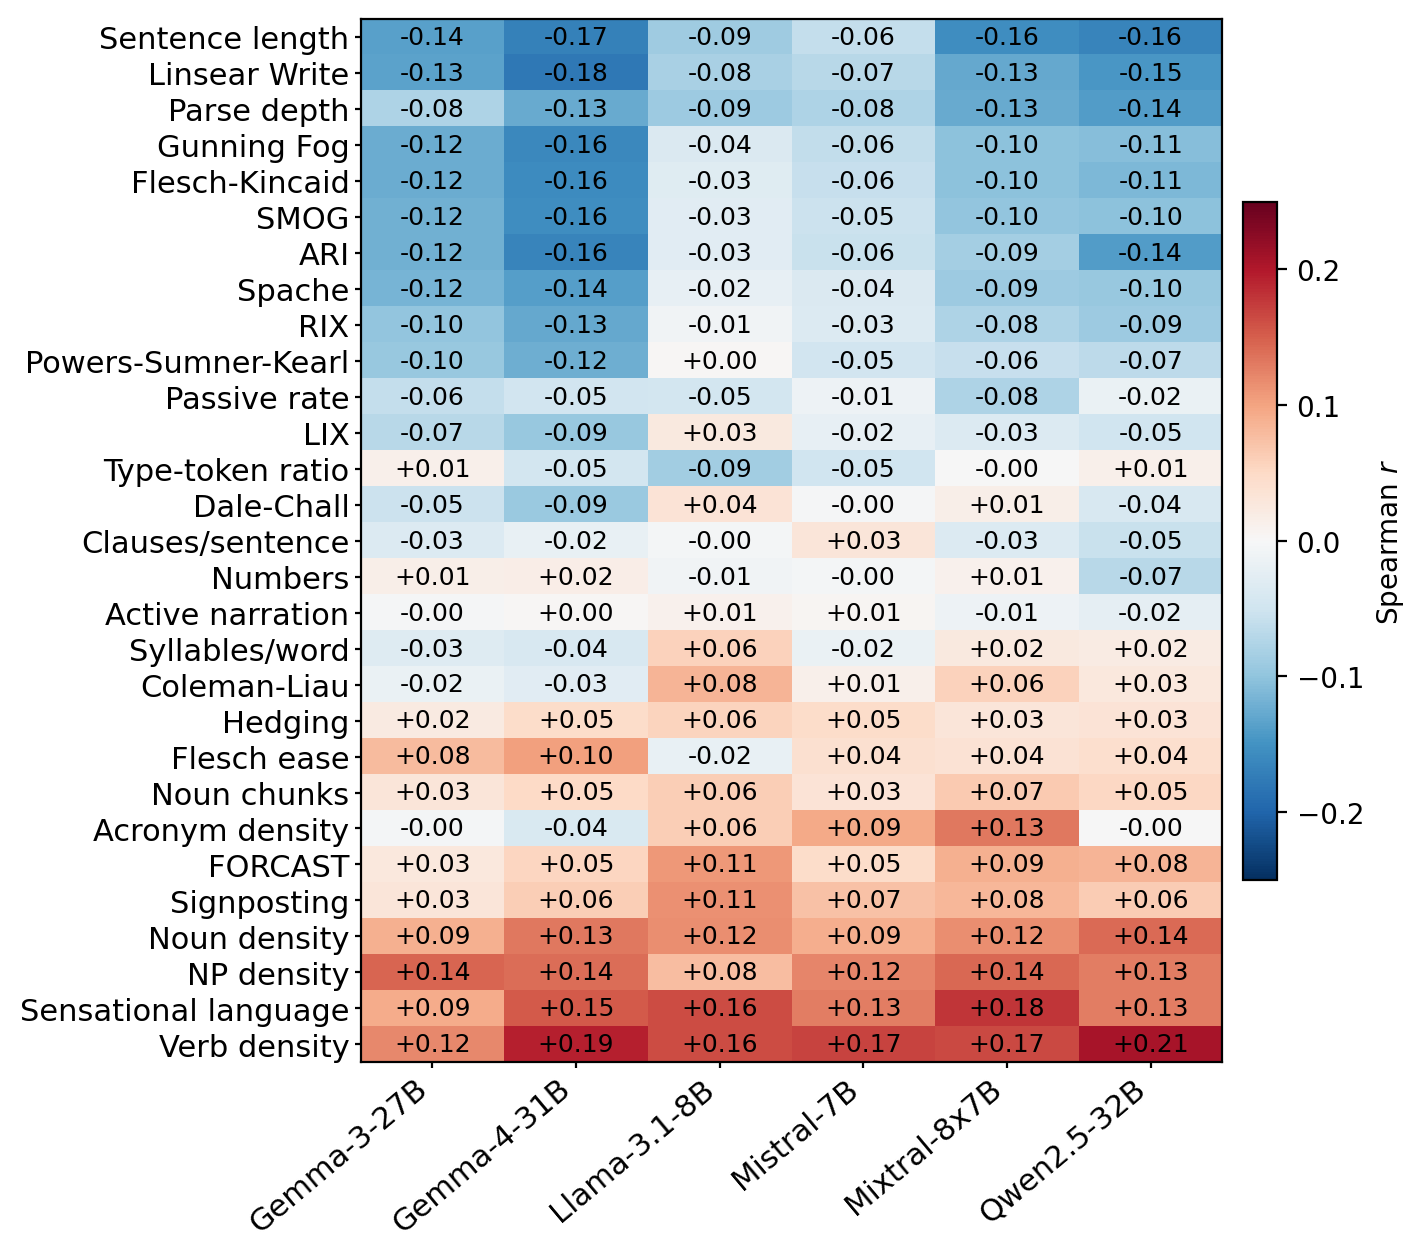
\includegraphics[width=0.72\textwidth]{figs/fig_judge_metric_heatmap.png}
\caption{\textbf{Per-paper correlation between writing metrics and judge
  score.} Spearman
  correlation between each writing metric and each model's judge score, over
  24,754 NeurIPS abstracts. A model's score for an abstract is the median of
  its nine generations, three prompts by three sampled runs. Rows are sorted
  by the correlation with the mean of those six per-model scores
  (1987--2024, the years the judge was scored). The judge score runs 1 to 5
  with higher meaning easier, so each cell's sign says which way that feature
  moves the judge. \textbf{Red (positive): more of that feature is judged
  \emph{more} readable}, as for verb density, sensational language and noun
  phrase density. \textbf{Blue (negative): more of it is judged \emph{less}
  readable}, as for sentence length and syntactic complexity, which is the
  direction the classical formulas also take. Near-white cells, including
  acronym density, indicate near indifference. All values are Spearman
  correlations and every effect is small ($|r| < 0.25$).}
\label{fig:judge-tracks}
\end{figure*}
